\documentclass{article}
\usepackage{tikz}
\usepackage{tkz-euclide}
\definecolor{darkgreen}{RGB}{0,192,0}
\title{Cartesian closed categories and the price of eggs}
\author{Jane Doe}
\date{September 1994}
\begin{document}

\newcommand*\circled[1]{\tikz[baseline=(char.base)]{
            \node[shape=circle,draw] (char) {#1};}}

\begin{figure}
	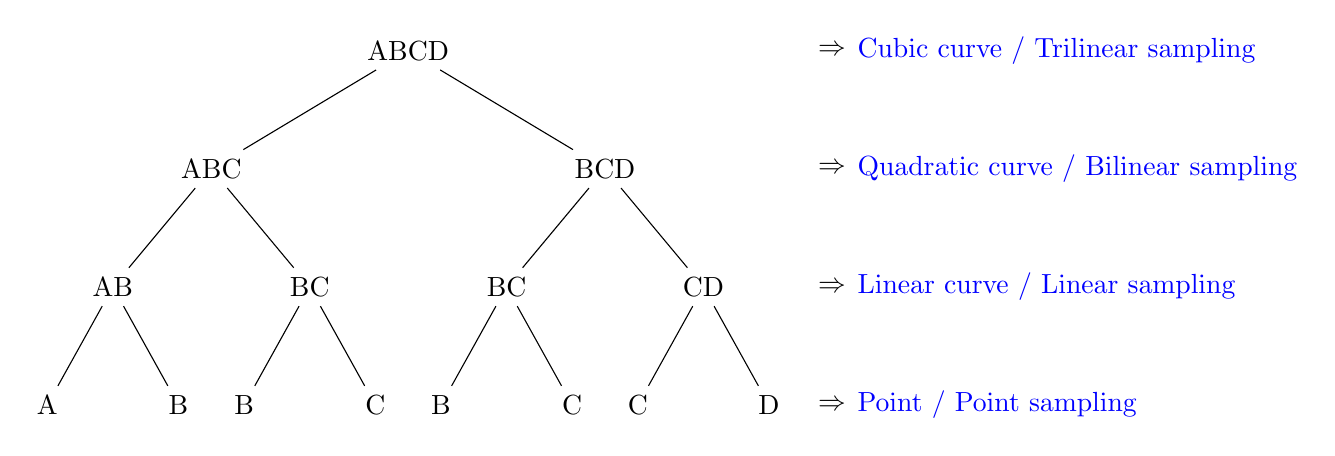
\begin{tikzpicture}[level/.style={sibling distance = 5cm/#1, level distance = 1.5cm}] 
		\begin{scope}[shift={(-6cm,0)}]
			\node (Root) {\circled{ABCD}}
			    child{ node{\circled{ABC}}
			            child{ node {\circled{AB}}
			            	child{ node {\circled{A}}}
			            	child{ node {\circled{B}}}            
			            }
			            child{ node {\circled{BC}}
			            	child{ node {\circled{B}}}
			            	child{ node {\circled{C}}}            
			            }                            
			    }
			    child{ node {\circled{BCD}}
			            child{ node {\circled{BC}}
			            	child{ node {\circled{B}}}
			            	child{ node {\circled{C}}}
			            }  
			            child{ node {\circled{CD}}
			            	child{ node {\circled{C}}}
			            	child{ node {\circled{D}}}
			            }  
					}
			; 

			% Comments for each level
			\begin{scope}[every node/.style={right}]
				\path (Root      -| Root-2-2-2) ++(5mm,0) node {$\Rightarrow$} ++(5mm,0) node [blue] {Cubic curve / Trilinear sampling};
				\path (Root-1    -| Root-2-2-2) ++(5mm,0) node {$\Rightarrow$} ++(5mm,0) node [blue] {Quadratic curve / Bilinear sampling};
				\path (Root-1-1  -| Root-2-2-2) ++(5mm,0) node {$\Rightarrow$} ++(5mm,0) node [blue] {Linear curve / Linear sampling};
				\path (Root-1-1-1-| Root-2-2-2) ++(5mm,0) node {$\Rightarrow$} ++(5mm,0) node [blue] {Point / Point sampling};
			\end{scope}
		\end{scope}   
	\end{tikzpicture}
	\caption{A tree showing the De Casteljeau algorithm for a cubic curve.  The labels on the right show what type of curves are evaluated at that level, as well as the $N$ dimensional sampling that is required to evaluate nodes at that level with a single texture read.}
\end{figure}		

\end{document}